% ============================================================
% QUDA MultiGrid 理解与 PyQCU 复现 — 2026-08-30 性能/显存补充汇报
% 编译：xelatex 两遍；交付闸门：Overfull=0, Float too large=0
% ============================================================
% 版式账本（逐页 map）：
% F1 title | 极简标题 | 16:9 | 风险：无
% F2 claim-conclusion | 三栏状态卡+流程 | 0.93\linewidth | min=\small
% F3 claim-quda-control | 单列算法表+流程 | 0.95\linewidth | min=\footnotesize
% F4 claim-transfer-coarse | 方程+映射表 | 0.94\linewidth | min=\footnotesize
% F5 claim-parity | 方程+流程 | 0.94\linewidth | min=\small
% F6 claim-precondition | 单列 V-cycle+比较表 | 0.94\linewidth | min=\footnotesize
% F7 claim-pyqcu-map | 新旧实现映射表 | 0.95\linewidth | min=\footnotesize
% F8 claim-local-stencil | 单列 setup 工作流 | 0.94\linewidth | min=\footnotesize
% F9 claim-memory | 复杂度公式+结果表 | 0.94\linewidth | min=\footnotesize
% F10 claim-results | setup benchmark 结果表 | 0.95\linewidth | min=\footnotesize
% F11 claim-validation | 分布式/混合精度验证矩阵 | 0.95\linewidth | min=\scriptsize
% F12 claim-risk | 风险/边界表 | 0.95\linewidth | min=\footnotesize
% F13 claim-next | 结论+下一步时间线 | 0.94\linewidth | min=\small
% F14 appendix-source | 源码索引+命令 | 0.95\linewidth | min=\scriptsize
% F15 appendix-gates | 验证命令+交付闸门 | 0.95\linewidth | min=\scriptsize

\documentclass[UTF8,aspectratio=169,11pt]{ctexbeamer}

\usepackage{amsmath,amssymb}
\usepackage{booktabs}
\usepackage{tabularx}
\usepackage{array}
\usepackage{tikz}
\usetikzlibrary{arrows.meta,positioning,calc,fit,shapes.geometric}
\usepackage{listings}
\usepackage{xcolor}
\usepackage{microtype}
\usepackage{hyperref}

\definecolor{primary}{HTML}{17365D}
\definecolor{accent}{HTML}{1F77B4}
\definecolor{evidence}{HTML}{1E8449}
\definecolor{warning}{HTML}{C55A11}
\definecolor{muted}{HTML}{5B6573}
\definecolor{panel}{HTML}{F4F7FA}
\definecolor{violet}{HTML}{6C4A9E}
\definecolor{good}{HTML}{EAF5EE}
\definecolor{warnbg}{HTML}{FFF4E8}

\setbeamersize{text margin left=0.55cm,text margin right=0.55cm}
\setlength{\columnsep}{0.28cm}
\setlength{\emergencystretch}{2em}
\setbeamertemplate{navigation symbols}{}
\setbeamertemplate{blocks}[rounded][shadow=false]
\setbeamercolor{normal text}{fg=black!86,bg=white}
\setbeamercolor{structure}{fg=primary}
\setbeamercolor{frametitle}{fg=primary,bg=white}
\setbeamercolor{block title}{fg=primary,bg=panel}
\setbeamercolor{block body}{fg=black!86,bg=panel}
\setbeamercolor{alerted text}{fg=warning}
\setbeamerfont{frametitle}{size=\large,series=\bfseries}
\setbeamerfont{normal text}{size=\normalsize}
\setbeamertemplate{frametitle}{\vskip0.12cm\insertframetitle\par\vskip0.08cm}
\setbeamertemplate{footline}{%
  \hbox{\begin{beamercolorbox}[wd=\paperwidth,ht=2.3ex,dp=0.9ex,
    leftskip=0.55cm,rightskip=0.55cm]{author in head/foot}%
    \scriptsize\color{muted}\insertshortauthor\hfill
    \insertshorttitle\hfill\insertframenumber/\inserttotalframenumber
  \end{beamercolorbox}}}

\newcolumntype{Y}{>{\raggedright\arraybackslash}X}
\newcolumntype{P}[1]{>{\raggedright\arraybackslash}p{#1}}
\newcommand{\source}[1]{%
  \vspace{0.03em}\par{\raggedright\fontsize{5.5pt}{6.5pt}\selectfont
  \color{muted}来源：#1\par}}
\newcommand{\codepath}[1]{%
  \ifmmode\text{\nolinkurl{#1}}\else\nolinkurl{#1}\fi}
\newcommand{\verified}{\textcolor{evidence}{确证}}
\newcommand{\inferred}{\textcolor{accent}{推断}}
\newcommand{\unverified}{\textcolor{warning}{未验证}}

\tikzset{
  flow/.style={draw=accent,fill=accent!8,rounded corners=2pt,align=center,
    minimum height=0.56cm,text width=2.08cm,font=\small},
  state/.style={draw=primary,fill=primary!7,rounded corners=2pt,align=center,
    minimum height=0.56cm,text width=2.40cm,font=\small},
  phase/.style={draw=violet,fill=violet!8,rounded corners=2pt,align=center,
    minimum height=0.52cm,text width=2.10cm,font=\small},
  decision/.style={draw=warning,fill=warning!10,diamond,aspect=2.0,
    align=center,inner sep=1.2pt,font=\small},
  arrow/.style={-{Latex[length=2mm]},draw=primary,semithick},
  relation/.style={-{Latex[length=1.7mm]},draw=muted,thin,dashed},
  labelstyle/.style={font=\scriptsize,inner sep=1.5pt,fill=white,text=muted}
}

\lstset{
  basicstyle=\ttfamily\scriptsize,
  backgroundcolor=\color{panel},frame=single,
  breaklines=true,breakatwhitespace=false,keepspaces=true,
  columns=flexible,numbers=left,numberstyle=\tiny\color{muted},
  keywordstyle=\color{primary}\bfseries,
  commentstyle=\color{evidence!70!black},stringstyle=\color{accent}
}

\title[QUDA MG 复现与优化]{QUDA MultiGrid 的算法理解与 PyQCU 复现}
\subtitle{MATPC 紧凑 odd Schur、P/R、Clover/Gauge、33 点粗算子与 setup 优化}
\author[代码审计与代数验证]{代码审计与代数验证}
\institute{PyQCU · Lattice QCD}
\date{2026 年 8 月 30 日}

\begin{document}

\begin{frame}[plain]
  \titlepage
\end{frame}

\begin{frame}[t]{本阶段结论：代数闭环与 MPI 闸门通过，setup 进入批量/显存优化}
  \small
  \begin{columns}[T,totalwidth=\textwidth]
    \begin{column}{0.30\textwidth}
      \begin{block}{已完成}
        QUDA 风格 MATPC：细层一次 odd Schur；粗层直接
        $R D P$。P/R、Clover/Gauge、33 点 stencil、V-cycle、重构与旧实现对照均已落地。
      \end{block}
    \end{column}
    \begin{column}{0.30\textwidth}
      \begin{block}{本轮证据}
        批量局部探测相对逐点为
        $0.155\,\mathrm{s}\to0.122\,\mathrm{s}$，约 $1.266\times$，最大差为 0；
        2/4 rank parity 回环最大差为 0。
      \end{block}
    \end{column}
    \begin{column}{0.30\textwidth}
      \begin{alertblock}{资源策略}
        Schur 窗口矩阵按方向流式切片；工作区不足时当前批次自动减半重试。
        旧缺陷路径保留，不做无声替换。
      \end{alertblock}
    \end{column}
  \end{columns}
  \vspace{0.20em}
  \begin{center}
    \begin{tikzpicture}[node distance=0.16cm and 0.18cm]
      \node[flow] (d) {完整 $D_f$};
      \node[flow,right=of d] (s) {一次 $S_o$};
      \node[flow,right=of s] (p) {$P_0,R_0$};
      \node[flow,right=of p] (g) {$R_0S_oP_0$};
      \node[flow,right=of g] (r) {递归 V-cycle};
      \draw[arrow] (d)--(s)--(p)--(g)--(r);
    \end{tikzpicture}
  \end{center}
  \vspace{0.18em}
  \colorbox{good}{\parbox{0.91\textwidth}{\textbf{阶段判断：}
    关键不变量已经可测：奇偶布局保持、$R=P^\dagger$、粗算子保留 local 与 hopping、
    分布式 33 点 halo 与混合精度运行不破坏真残差；当前主要瓶颈从正确性转为 setup 成本。}}
  \source{实现：\codepath{pyqcu/solver/_quda_multigrid.py:1094-1292,1691-2331}；
    优化：\codepath{pyqcu/tools/_multigrid.py:938-1334}；
    测试：\codepath{examples/qcu/dev87/}。}
\end{frame}

\begin{frame}[t]{QUDA 的递归控制流：reset 建层，operator 做一次完整 V-cycle}
  \footnotesize
  \begin{columns}[T,totalwidth=\textwidth]
    \begin{column}{0.52\textwidth}
      \begin{tabular}{@{}l@{}}
        $\text{输入： }D_\ell,\;B_\ell,\;\text{aggregate geometry},\;\text{precision}$\\
        $\text{reset：生成/刷新 }B_\ell\text{ 与 Transfer}_\ell$\\
        $\quad B_{\ell+1,i}\leftarrow R_\ell B_{\ell,i}$\\
        $\text{createCoarseDirac： }D_{\ell+1}=R_\ell D_\ell P_\ell$\\
        $\quad\text{分别保存 residual、smoother 与 sloppy operator}$\\
        $\text{createCoarseSolver：封装 coarse solver 与递归 MG}$\\
        $\text{operator：prepare}\to\text{pre-smooth}\to Rr\to\text{recurse}$\\
        $\quad\to Pe_c\to\text{post-smooth}$\\
        $\text{输出：solution；若类型不同则 reconstruct 后重算 residual}$
      \end{tabular}
    \end{column}
    \begin{column}{0.38\textwidth}
      \begin{tikzpicture}[node distance=0.12cm]
        \node[state,font=\scriptsize,text width=2.55cm] (a) {细格 Dirac 与 $B$};
        \node[state,font=\scriptsize,text width=2.55cm,below=of a] (b) {Transfer / $RDP$};
        \node[state,font=\scriptsize,text width=2.55cm,below=of b] (c) {$X,Y$ 与 solver wrapper};
        \node[state,font=\scriptsize,text width=2.55cm,below=of c] (d) {递归 coarse MG};
        \draw[arrow] (a)--(b)--(c)--(d);
        \draw[relation] (d.east) -- ++(0.40,0) |- node[right=1pt,labelstyle]{返回校正}
          (b.east);
      \end{tikzpicture}
      \vspace{0.20em}
      \begin{block}{控制流含义}
        \scriptsize
        粗化只改变表示空间；每一级仍有完整 operator、平滑器、残差和停止判据。
        因而“粗层只有 dslash”不等价于 QUDA 的 coarse Dirac。
      \end{block}
    \end{column}
  \end{columns}
  \vspace{0.14em}
  \begin{center}
    \begin{tikzpicture}[node distance=0.20cm and 0.30cm]
      \node[phase] (x) {细层 $D_\ell$};
      \node[phase,right=of x] (v) {$P_\ell$ 延拓};
      \node[phase,right=of v] (r) {$D_\ell$ 作用};
      \node[phase,right=of r] (q) {$R_\ell$ 限制};
      \node[phase,right=of q] (y) {粗层 $D_{\ell+1}$};
      \draw[arrow] (x)--(v)--(r)--(q)--(y);
    \end{tikzpicture}
  \end{center}
  \source{QUDA：\codepath{refer/git-rep/quda/lib/multigrid.cpp:72-197,1131-1224}；
    PyQCU：\codepath{pyqcu/solver/_quda_multigrid.py:1915-1986}。}
\end{frame}

\begin{frame}[t]{P/R 与粗算子：局部正交化与 $RDP$ 缺一不可}
  \footnotesize
  \begin{columns}[T,totalwidth=\textwidth]
    \begin{column}{0.44\textwidth}
      \begin{block}{Transfer 的物理/代数定义}
        \begin{align*}
          a(x)&=\left(\left\lfloor x_0/b_0\right\rfloor,\ldots,
          \left\lfloor x_3/b_3\right\rfloor\right),\\
          (P\eta)_{sc}(x)&=\sum_jV_{scqj}(x)\eta_{qj}(a(x)),\\
          (R\psi)_{qj}(a)&=\sum_{x\in a,s,c}V^*_{scqj}(x)\psi_{sc}(x),\\
          R&=P^\dagger,\qquad RP\simeq I_c.
        \end{align*}
        Wilson/Clover 的细自由度为 $D_f=4\times3=12$；每个 aggregate 内
        的 block CGS 产生 coarse vectors $V$。
      \end{block}
    \end{column}
    \begin{column}{0.46\textwidth}
      \begin{tabularx}{0.96\linewidth}{@{}P{0.25\linewidth}Y@{}}
        \toprule
        对象 & 在 $RDP$ 中的作用 \\
        \midrule
        Gauge $U_\mu$ & 进入 Wilson forward/backward hopping；方向、边界和伴随决定 $Y^\pm$。\\
        Clover $C$ & 进入 local diagonal block $X$；$X^{-1}$ 参与 Schur 与预条件。\\
        local block & $X(q)=V^\dagger D_{\rm local}V$，不是可省略的装饰项。\\
        hopping block & $Y^\pm(q)=V^\dagger D_{\rm hop}V$，保留传播方向。\\
        coarse stencil & $1+8+24=33$ 个本点、轴邻居和二维对角邻居。\\
        \bottomrule
      \end{tabularx}
    \end{column}
  \end{columns}
  \vspace{0.16em}
  \begin{center}
    \begin{tikzpicture}[node distance=0.25cm and 0.28cm]
      \node[flow] (b) {fine block $b$};
      \node[flow,right=of b] (v) {局部 $V$};
      \node[flow,right=of v] (d) {Clover + Gauge $D$};
      \node[flow,right=of d] (c) {coarse $X,Y$};
      \draw[arrow] (b)--node[above=1pt,labelstyle]{$\mathrm{CGS/QR}$}(v);
      \draw[arrow] (v)--node[above=1pt,labelstyle]{$V^\dagger D V$}(d);
      \draw[arrow] (d)--(c);
    \end{tikzpicture}
  \end{center}
  \begin{alertblock}{极限检查}
    \scriptsize
    若 coarse vectors 超过 aggregate 的局部维数，$RP\simeq I_c$ 无法成立；
    若丢掉 $X$ 或 $Y$，分别改变局部质量/磁场耦合或传播，不能称为完整粗算子。
  \end{alertblock}
  \source{QUDA：\codepath{refer/git-rep/quda/lib/transfer.cpp:200-328}、
    \codepath{refer/git-rep/quda/lib/coarse_op.cuh:1035-1459}；
    PyQCU：\codepath{pyqcu/solver/_quda_multigrid.py:664-1056}。}
\end{frame}

\begin{frame}[t]{奇偶处理：MATPC 首层形成 odd Schur，粗层不再重复 checkerboard}
  \footnotesize
  \begin{columns}[T,totalwidth=\textwidth]
    \begin{column}{0.48\textwidth}
      \begin{block}{块矩阵与重构}
        \begin{equation*}
          D=\begin{pmatrix}D_{ee}&D_{eo}\\D_{oe}&D_{oo}\end{pmatrix},
          \qquad S_o=D_{oo}-D_{oe}D_{ee}^{-1}D_{eo}.
        \end{equation*}
        \begin{align*}
          b_o^S&=b_o-D_{oe}D_{ee}^{-1}b_e,\\
          S_ox_o&=b_o^S,\\
          x_e&=D_{ee}^{-1}(b_e-D_{eo}x_o).
        \end{align*}
        $D_{ee}$ 的 Clover/local block 必须可逆；$D^\dagger$ 路径需使用
        $(D_{ee}^{-1})^\dagger$，不能把 Schur 当作自动 Hermitian。
      \end{block}
    \end{column}
    \begin{column}{0.38\textwidth}
      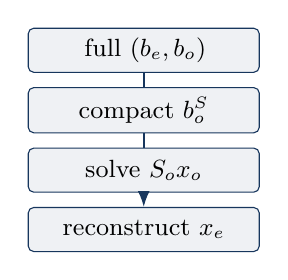
\begin{tikzpicture}[node distance=0.18cm]
        \node[state,text width=2.70cm] (a) {full $(b_e,b_o)$};
        \node[state,text width=2.70cm,below=of a] (b) {compact $b_o^S$};
        \node[state,text width=2.70cm,below=of b] (c) {solve $S_ox_o$};
        \node[state,text width=2.70cm,below=of c] (d) {reconstruct $x_e$};
        \draw[arrow] (a)--(b)--(c)--(d);
      \end{tikzpicture}
      \vspace{0.06em}
      \begin{alertblock}{一次减半原则}
        \scriptsize
        $D_f\to S_o$ 已将 parity 压进 odd compact geometry；
        $A_{\ell+1}=R_\ell A_\ell P_\ell$ 直接 Galerkin，不能再 Schur（否则 $T/4$）。
      \end{alertblock}
    \end{column}
  \end{columns}
  \vspace{0.04em}
  \begin{block}{紧凑布局的坐标关系}
    \scriptsize
    \begin{align*}
      p&=(x+y+z+t)\bmod2,\quad e_s=(x+y+z)\bmod2,\\
      t_{\rm full}&=2t_{\rm half}+((p-x-y-z)\bmod2).
    \end{align*}
    odd 页不是简单奇数 $t$ 切片；$T$ 与各 local 物理轴须为偶数。
  \end{block}
  \source{QUDA：\codepath{refer/git-rep/quda/lib/multigrid.cpp:347-434,1131-1224}；
    QCU：\codepath{cpp/cuda/qcu/src/multigrid.cu:1579-1743}；
    PyQCU：\codepath{pyqcu/solver/_quda_multigrid.py:1094-1370}。}
\end{frame}

\begin{frame}[t]{预条件与 V-cycle：$X^{-1}$ 改善局部尺度，但不删除完整 $D_c$}
  \scriptsize
  \begin{columns}[T,totalwidth=\textwidth]
    \begin{column}{0.48\textwidth}
      \begin{block}{粗层预条件的代数链}
        \begin{align*}
          D_c&=X+H,\\
          D_{\rm pc}&=X^{-1}(D_c-X)=X^{-1}H,\\
          D_{\rm full,pc}&=X^{-1}D_c=I+D_{\rm pc},\\
          \widehat Y^+_\mu(q)&=X^{-1}(q)Y^+_\mu(q).
        \end{align*}
        backward link 要同时处理存储位置平移、伴随和右侧
        $X^{-\dagger}$ 约定；只检查 forward 不足以证明 PC 算子正确。
      \end{block}
    \end{column}
    \begin{column}{0.42\textwidth}
      \begin{tabular}{@{}P{0.98\linewidth}@{}}
        $r_\ell=b_\ell-A_\ell x_\ell$ \\
        $x_\ell\leftarrow\mathrm{smooth}(A_\ell,r_\ell)$ \\
        $r_{\ell+1}\leftarrow R_\ell r_\ell$ \\
        $e_{\ell+1}\leftarrow\mathrm{solve}(A_{\ell+1},r_{\ell+1})$ \\
        $x_\ell\leftarrow x_\ell+P_\ell e_{\ell+1}$ \\
        $x_\ell\leftarrow\mathrm{smooth}(A_\ell,r_\ell,x_\ell)$ \\
        $K(r_\ell)=x_\ell$ 作为外层 FGMRES/BiCGStab 预条件器
      \end{tabular}
      \vspace{0.18em}
      \begin{block}{实现分离}
        \scriptsize
        QUDA 同时维护 residual operator、smoother operator 与 sloppy precision；
        PyQCU 对应 \codepath{preconditioned_apply}、\codepath{v_cycle} 与显式 true residual。
      \end{block}
    \end{column}
  \end{columns}
  \vspace{0.04em}
  \source{QUDA：\codepath{refer/git-rep/quda/include/kernels/coarse_op_preconditioned.cuh}、
    \codepath{refer/git-rep/quda/lib/dirac_coarse.cpp:351-430,506-626}；
    PyQCU：\codepath{pyqcu/solver/_quda_multigrid.py:912-1056,2021-2034}。}
\end{frame}

\begin{frame}[t]{PyQCU 的新旧实现边界：新路径复现 QUDA 代数，旧路径作为缺陷对照保留}
  \footnotesize
  \begin{center}
    \renewcommand{\arraystretch}{0.94}
    \begin{tabularx}{0.95\textwidth}{@{}P{0.22\textwidth}P{0.34\textwidth}Y@{}}
      \toprule
      维度 & 新实现：\texttt{QudaMultigrid + CompactParityOperator} & 旧实现：\texttt{solver.multigrid} \\
      \midrule
      finest operator & 完整 Wilson/Clover $D_f$，一次形成 $S_o$ & MG-0 有奇偶处理，但接口与新 compact 层级分离 \\
      coarse parity & 当前 odd compact geometry 上直接 $RDP$，不重复减半 & 粗层没有对应的完整 parity 递归约束 \\
      coarse operator & $X$ local block + $Y^\pm$ hopping，支持 33 点 stencil & 粗层算子为不完备的 hopping/dslash 近似 \\
      P/R & aggregate-local block orthogonalization，$R=P^\dagger$ & 历史接口，不能作为 QUDA 等价性证据 \\
      solve & V/W/F/K-cycle、smoother、reconstruct、true residual & 作为历史/缺陷实现和对照基线 \\
      \bottomrule
    \end{tabularx}
  \end{center}
  \vspace{0.04em}
  \begin{columns}[T,totalwidth=\textwidth]
    \begin{column}{0.46\textwidth}
      \begin{block}{层级协议}
        \scriptsize
        $A_0=D_f,\ A_1=R_0S_oP_0,\ 
        A_{\ell+1}=R_\ell A_\ell P_\ell\ (\ell\ge1)$。
        这就是“只在 finest 做 Schur”。
      \end{block}
    \end{column}
    \begin{column}{0.42\textwidth}
      \begin{alertblock}{工程边界}
        \scriptsize
        新 API 通过 compact/full round-trip、Galerkin 和 QCU asset shape；
        旧实现保留作缺陷对照，不删除、不暗中替换。
      \end{alertblock}
    \end{column}
  \end{columns}
  \source{新实现与旧实现的完整源码索引见附录；对照矩阵为
    \texttt{examples/qcu/dev87/comparison\_matrix.md}。}
\end{frame}
\begin{frame}[t]{局部 33 点 stencil setup：用有限传播半径替代全格 Schur 探测}
  \scriptsize
  \begin{center}
    \begin{tabular}{@{}l@{}}
      $\text{输入： }\text{fine Schur components},\;\text{local orthogonal }V,\;W=10,\;E$\\
      $\text{按粗点 }c\text{ 建窗口： }x_0=2c-(W/2-1)，\text{在中心块填充 }E\text{ 个单位探针}$\\
      $\text{局部 action： }f_c\xrightarrow{D_{oe}}D_{ee}^{-1}\xrightarrow{D_{eo}}S_of_c$\\
      $\text{限制：仅取 }c\text{ 本点、4 轴邻居和 24 个二维对角块，计算 }V^\dagger S_oV$\\
      $\text{写回： }sit,\;hop\_nn,\;hop\_diag\text{；周期退化或窗口不足时回退逐点参考路径}$\\
      $\text{输出： }[E,E,X_c,Y_c,Z_c,T_c]\;+\;[2,4,E,E,\cdots]\;+\;[2,2,6,E,E,\cdots]$
    \end{tabular}
  \end{center}
  \vspace{0.04em}
  \begin{columns}[T,totalwidth=\textwidth]
    \begin{column}{0.47\textwidth}
      \begin{block}{为什么窗口足够}
        \begin{align*}
          \mathrm{supp}(D)&:\;1\text{ 个轴向 hop},\\
          \mathrm{supp}(S_o)&:\;\text{两次 hop + local inverse},\\
          \mathrm{supp}(R S_oP)&:\;c\pm1\text{ 块与二维对角块}.
        \end{align*}
        $W=10$ 给中心块外侧 padding，周期边界用坐标模运算保持连续切片语义。
      \end{block}
    \end{column}
    \begin{column}{0.41\textwidth}
      \begin{tikzpicture}[node distance=0.16cm]
        \node[phase] (a) {全格探测};
        \node[phase,below=of a] (b) {局部 $W^4$ 窗口};
        \node[phase,below=of b] (c) {33 块 restriction};
        \node[phase,below=of c] (d) {HDF5 coarse asset};
        \draw[arrow] (a)--(b)--(c)--(d);
      \end{tikzpicture}
      \vspace{0.12em}
      \begin{block}{支撑边界}
        \scriptsize
        更宽 operator 必须扩展窗口与 C++ kernel，禁止静默截断。
      \end{block}
    \end{column}
  \end{columns}
  \source{实现：\codepath{pyqcu/tools/_multigrid.py:990-1277}；
    参考日志：\codepath{logs/v20260818.txt}。}
\end{frame}

\begin{frame}[t]{本轮性能/显存优化：计算批量化，同时把窗口矩阵从“全驻留”改为流式}
  \footnotesize
  \begin{columns}[T,totalwidth=\textwidth]
    \begin{column}{0.45\textwidth}
      \begin{block}{峰值内存的量纲估算}
        旧路径在一次 Schur 调用前物化 18 组窗口矩阵：
        \begin{equation*}
          M_{\rm old}=18K\cdot12\cdot12\cdot W^4\cdot s_{\rm cplx}.
        \end{equation*}
        $W=10,K=4$ 时，$M_{\rm old}=0.829\,\mathrm{GB}$（c64），
        $1.659\,\mathrm{GB}$（c128），尚未计入 Schur work buffers。
      \end{block}
      \begin{block}{新路径}
        每个方向只保留 source、一个矩阵窗口和一次 contraction temporary；
        $D_{ee}^{-1}$、$D_{oo}$ 分阶段切片，并在 restrict 前释放局部场。
      \end{block}
    \end{column}
    \begin{column}{0.45\textwidth}
      \begin{tabularx}{0.98\linewidth}{@{}P{0.31\linewidth}Y@{}}
        \toprule
        措施 & 工程效果 \\
        \midrule
        K 批量 & $K$ 个互不相交窗口一次调度，减少 Python/CUDA launch 与切片开销。\\
        流式矩阵 & 18 份矩阵不再同时存活，峰值随当前方向而非 18 组增长。\\
        及时释放 & \codepath{f_local}、$D_{\rm local}$、restrict 临时在生命周期末立即释放。\\
        OOM retry & 当前批次按 $K\to\lceil K/2\rceil$ 重试，已写点不重复写。\\
        \bottomrule
      \end{tabularx}
      \vspace{0.18em}
      \begin{alertblock}{可调旋钮}
        \scriptsize
        \codepath{build_stencil_local(..., batch_size=4)} 默认批量；显存紧张可传更小
        $K$，异常时自动降档，不改变 $R S_oP$ 数学结果。
      \end{alertblock}
    \end{column}
  \end{columns}
  \source{实现：\codepath{pyqcu/tools/_multigrid.py:938-987,1026-1067,1166-1240,1279-1334}；
    测量命令：\codepath{examples/qcu/dev87/test_stencil_batch_local.py} 与本轮 CPU benchmark。}
\end{frame}

\begin{frame}[t]{当前实测：批量局部探测保持逐点结果，并降低 setup 调度成本}
  \scriptsize
  \begin{center}
    \renewcommand{\arraystretch}{1.06}
    \begin{tabularx}{0.95\textwidth}{@{}P{0.20\textwidth}P{0.20\textwidth}P{0.17\textwidth}P{0.16\textwidth}Y@{}}
      \toprule
      验证项 & 参考/配置 & 当前结果 & 误差/状态 & 判读 \\
      \midrule
      流式 Schur vs 物化公式 & 随机非对角矩阵、$K=4$ & shape 一致 & max abs $=0$ & contraction 顺序与 parity mask 保持 \\
      局部 stencil K=1 vs K=4 & fine $8^4$、coarse $4^4$、$E=3$ & 逐点/批量 & max diff $=0$ & 周期边界和内部粗点均覆盖 \\
      CPU batch benchmark & $E=2,W=6$、4 个粗点 & $0.155\to0.122$ s & $1.266\times$ & 仅计 setup 探测，非 GPU 吞吐声明 \\
      Python 主回归 & \texttt{pytest -q examples/pyqcu} & 26 passed & exit 0 & 既有代数/solver 行为未回归 \\
      breakdown guard & zero coarse operator & 2 passed & finite output & 粗求解 breakdown 不污染细解 \\
      \bottomrule
    \end{tabularx}
  \end{center}
  \vspace{0.08em}
  \begin{columns}[T,totalwidth=\textwidth]
    \begin{column}{0.45\textwidth}
      \begin{block}{数值不变量}
        \scriptsize
        流式 action 与物化参考逐元素相同；K 批量只改变独立窗口的执行顺序，
        不改变中心点与 33 个目标块的写集。
      \end{block}
    \end{column}
    \begin{column}{0.45\textwidth}
      \begin{alertblock}{口径}
        \scriptsize
        CPU benchmark 用于证明调度收益和等价性；完整 GPU/MPI 性能仍需在目标设备和
        固定数据缓存下单独测量，不能从该数字外推 QUDA 原生吞吐。
      \end{alertblock}
    \end{column}
  \end{columns}
  \source{测试：\codepath{examples/qcu/dev87/test_stencil_batch_local.py}、
    \codepath{examples/qcu/dev87/test_mg_breakdown.py}；
    命令：\codepath{pytest -q examples/qcu/dev87/test_stencil_batch_local.py examples/qcu/dev87/test_mg_breakdown.py}。}
\end{frame}

\begin{frame}[t]{分布式与混合精度验证：奇偶、粗 halo 和真残差均有独立证据}
  \scriptsize
  \begin{center}
    \renewcommand{\arraystretch}{1.04}
    \begin{tabularx}{0.96\textwidth}{@{}P{0.27\textwidth}P{0.24\textwidth}P{0.20\textwidth}Y@{}}
      \toprule
      路径 & 配置 & 实测指标 & 结论 \\
      \midrule
      compact parity round-trip & 2 rank $[2,1,1,1]$ c64；2 rank $[1,1,1,2]$ c128 & global max/rel $=0$ & $T/2$ 页按物理坐标重建正确 \\
      compact parity round-trip & 4 rank $[1,2,1,2]$ c64；$[1,1,2,2]$ c128 & global max/rel $=0$ & X/Y/Z/T rank 原点均覆盖 \\
      distributed coarse equivalence & 2 rank、c64、$[2,1,1,1]$ & global L2 rel $=5.60\times10^{-7}$ & 33 点周期 halo 与全局参考一致 \\
      distributed coarse equivalence & 2 rank、c128、$[1,1,1,2]$ & global L2 rel $=1.03\times10^{-15}$ & 双精度路径一致 \\
      coarse dslash smoke & 2 rank、host staging、overlap off & rel max $=0$ & 无死锁/非法访问 \\
      end-to-end MG & 2 rank、fine c64/coarse c128 & true residual rel $\simeq7.69\times10^{-7}$ & 混合精度粗层可运行 \\
      \bottomrule
    \end{tabularx}
  \end{center}
  \vspace{0.04em}
  \begin{block}{MPI 设计判断}
    \scriptsize
    parity 页不能直接按压缩轴切块；先恢复物理格点、切 rank block、再压缩。
    粗层不做 checkerboard，但保留本 rank 的 33 点 stencil，并对跨 rank 的 32 个邻居做 halo。
  \end{block}
  \source{回环：\codepath{examples/qcu/dev87/parity_mpi_roundtrip.py:48-118}；
    粗算子：\codepath{examples/qcu/dev87/coarse_mpi_equiv.py:46-122}；
    MG：\codepath{examples/qcu/dev87/run_qcu_mg_mpi.py:209-222}；命令证据：本轮 MPI 运行输出。}
\end{frame}

\begin{frame}[t]{当前限制与风险：正确性已闭环，生产性能仍受资产与通信口径约束}
  \footnotesize
  \begin{center}
    \renewcommand{\arraystretch}{1.08}
    \begin{tabularx}{0.95\textwidth}{@{}P{0.25\textwidth}P{0.30\textwidth}Y@{}}
      \toprule
      项目 & 已确证状态 & 仍需控制的风险/下一步 \\
      \midrule
      Schur window & $W=10$ 对当前 Wilson/Clover 33 点支撑等价；边界有回退 & 更宽 dslash、非局部项需重新证明传播半径并扩大窗口 \\
      setup memory & 矩阵切片流式化；K 批量工作区按需减半 & fine operator 的大体量 Clover/Gauge 资产仍是主显存项，应继续 VRAM$\to$RAM$\to$HDF5 分层 \\
      MPI halo & 2 rank 等价和 smoke 通过；当前为阻塞 host staging & 未测通信/计算 overlap、device-aware MPI 和 NVSHMEM 吞吐 \\
      mixed precision & c64/c128 coarse transition 与 true residual 通过 & 误差平台、更多层级和更大体积需固定设备复测 \\
      QUDA 性能对照 & 算法控制流/代数对象完成映射 & Python setup、QCU kernel、QUDA autotune/通信不是同一性能口径 \\
      legacy path & \codepath{pyqcu/solver/_multigrid.py} 保留作缺陷对照 & 使用新 API 时需显式选择，避免历史缓存与新 compact asset 混用 \\
      \bottomrule
    \end{tabularx}
  \end{center}
  \vspace{0.04em}
  \colorbox{warnbg}{\parbox{0.91\textwidth}{\textbf{风险控制：}
    所有“确证”只对应源码、恒等式或本轮命令输出；CPU batch 加速不外推 GPU；
    2/4 rank 正确性不外推强 scaling；未测项目保持“未验证”。}}
  \source{边界实现：\codepath{pyqcu/tools/_multigrid.py:1192-1222,1314-1327}；
    历史资源分析：\codepath{logs/dev80_2/dev80_2_analy.md:57-74}；
    MPI 限制记录：\codepath{examples/qcu/dev87/dev87_report.md:375-390}。}
\end{frame}

\begin{frame}[t]{阶段结论与下一步：从“能复现”转向“可扩展 setup”}
  \small
  \begin{columns}[T,totalwidth=\textwidth]
    \begin{column}{0.30\textwidth}
      \begin{block}{已确认}
        \scriptsize
        \begin{tabular}{@{}P{0.98\linewidth}@{}}
          QUDA 主线：$B\to V\to P/R\to RDP$；\\
          $X$、$Y$、$X^{-1}$、$Yhat$ 属于同一粗算子体系；\\
          compact MATPC 只在 finest 做一次 odd Schur；\\
          粗层完整保留 stencil 与 parity-aware 维度协议。
        \end{tabular}
      \end{block}
    \end{column}
    \begin{column}{0.30\textwidth}
      \begin{block}{本轮交付}
        \scriptsize
        流式 \codepath{BatchedLocalSchur}、K 批量局部探测、OOM 降档重试；
        parity MPI round-trip 测试；流式/物化参考测试；
        本报告 \codepath{..._20260830.tex/.pdf}。
      \end{block}
      \begin{alertblock}{稳定性}
        \scriptsize
        build、Python、MPI coarse、MG breakdown 和混合精度闸门均为通过。
      \end{alertblock}
    \end{column}
    \begin{column}{0.30\textwidth}
      \begin{block}{下一阶段验收}
        \scriptsize
        \begin{tabular}{@{}P{0.98\linewidth}@{}}
          1. 记录真实 GPU peak memory 与 K 的曲线；\\
          2. 大格 setup 的分层驻留和 HDF5 cache；\\
          3. halo 通信与计算 overlap；\\
          4. 同数据/同容差的 QUDA kernel benchmark。
        \end{tabular}
      \end{block}
    \end{column}
  \end{columns}
  \vspace{0.28em}
  \begin{center}
    \begin{tikzpicture}[node distance=0.25cm and 0.24cm]
      \node[phase] (a) {代数 golden contract};
      \node[phase,right=of a] (b) {MPI/混合精度};
      \node[phase,right=of b] (c) {显存分层 setup};
      \node[phase,right=of c] (d) {设备感知 benchmark};
      \draw[arrow] (a)--(b)--(c)--(d);
    \end{tikzpicture}
  \end{center}
  \source{本轮证据：\codepath{examples/qcu/dev87/}；
    代码：\codepath{pyqcu/tools/_multigrid.py:938-1334}；
    数据读写目录：\codepath{/root/PyQCU/data}。}
\end{frame}

\appendix

\begin{frame}[t]{附录：对象—源码—证据索引}
  \scriptsize
  \begin{center}
    \renewcommand{\arraystretch}{0.88}
    \begin{tabularx}{0.96\textwidth}{@{}P{0.22\textwidth}P{0.38\textwidth}Y@{}}
      \toprule
      对象 & QUDA 对照 & PyQCU 当前证据 \\
      \midrule
      递归 MG & \codepath{lib/multigrid.cpp:72-197,1131-1224} & \codepath{QudaMultigrid.setup/v_cycle} \\
      geometry/spin map & \codepath{lib/transfer.cpp:200-257} & \codepath{QudaTransfer}，含 Wilson/Clover map \\
      P/R & \codepath{lib/transfer.cpp:259-328} & block CGS/QR、$R=P^\dagger$、compact round-trip \\
      coarse $X/Y$ & \codepath{lib/coarse_op.cuh:1035-1459} & lazy/materialized $RDP$、33 点资产 \\
      PC/Yhat & \codepath{lib/dirac_coarse.cpp:351-430,506-626} & local inverse、preconditioned apply \\
      parity & \codepath{lib/multigrid.cpp:1131-1224} & odd Schur、reconstruct、no repeated checkerboard \\
      compact map & \codepath{cpp/cuda/qcu/src/multigrid.cu:1579-1743} & \codepath{CompactParityLayout}、MPI round-trip \\
      setup optimization & \codepath{coarse_op.cuh} 的局部支撑思想 & \codepath{BatchedLocalSchur} 流式/K 批量/OOM retry \\
      旧实现 & 历史 PyQCU 路径 & \codepath{pyqcu/solver/_multigrid.py} 保留 \\
      \bottomrule
    \end{tabularx}
  \end{center}
  \vspace{0.04em}
  \begin{block}{证据等级}
    \verified：本轮命令、数值直测或代码恒等式；
    \inferred：控制流与物理/代数对象的一致性判断；
    \unverified：QUDA 原生 kernel 公平性能、device-aware overlap、NVSHMEM 与更大体积 setup 峰值。
  \end{block}
  \source{源码索引与日志：\codepath{logs/v20260818.txt}、\codepath{logs/v20260829.txt}。}
\end{frame}

\begin{frame}[t]{附录：本轮验证命令与交付闸门}
  \scriptsize
  \begin{tabularx}{0.96\textwidth}{@{}Y r@{}}
    \texttt{pytest -q examples/pyqcu} & \textbf{26 passed}\\
    \texttt{pytest -q examples/qcu/dev87/test\_stencil\_batch\_local.py
      examples/qcu/dev87/test\_mg\_breakdown.py}
      & \textbf{2 passed}\\
    \texttt{python -m py_compile}（核心工具与 dev87 脚本） & \textbf{通过}\\
    环境与 CUDA 后端构建（env + build） & \textbf{CUDA backend SUCCESS}\\
    MPI parity round-trip（2/4 rank） & \textbf{all max/rel = 0}\\
    MPI 粗算子等价与 smoke（2 rank） & \textbf{5.60e-7 / 1.03e-15 / 0}\\
    端到端 MG（2 rank，coarse c128） & \textbf{exit 0；true residual 7.69e-7}\\
    \texttt{git diff --check} & \textbf{通过}\\
  \end{tabularx}
  \vspace{0.24em}
  \begin{block}{交付判定}
    页面数、渲染页数和逐页检查数必须一致；报告中的性能数字区分
    CPU setup benchmark、CUDA/MPI 正确性和未验证的 QUDA 原生吞吐，不混用。
  \end{block}
  \source{文件与缓存：docs/report\_quda\_multigrid\_reproduction\_20260830.tex/.pdf；
    所有缓存读写遵循 /root/PyQCU/data。}
\end{frame}

\end{document}
